\chapter{Introduction}
\label{chap:introduction}

\section{Self-driving solutions}
Nowadays, self-driving cars gain more and more attention, both their technology and their effect on people's daily routines and their lives overall. Several articles are published every year about how these cars will change the way people commute to work, visit their friends or go on a family vacation. These articles often point out the decrease of the number of accidents, an optimized load of traffic and thus a reduced fuel consumption as the major advantages of this technology-to-come.

The release date of these cars, however, is still a matter of question. In 2015, Mark Fields, president and CEO of Ford at the time estimated their first fully autonomous car in 2020. 2 years later, at CES 2017 Nvidia announced that with the partnership of Audi they would develop a self-driving vehicle --- also, in market by 2020. Both of these statements are considered too ambitious guesses today, as there is a high probability that we need to wait for at least another decade for reliable fully autonomous vehicles to hit the roads. Claiming that there are no viable signs of these cars in traffic would be a false statement, as there are several companies who have been testing there vehicles on public roads for the last years, but these prototypes are very far from reliable products yet. The company that seems to be ahead of the competition in this race is Tesla. Their self-driving software is already in their products, but it still needs millions of hours of testing and the responsibility is still the driver's if an accident happens.

But why is this delay of release dates? One possible answer is that manufacturers have the tendency to exaggerate when asked about new products, and thus the users' need and the other competitors development speed urged them to make such estimations they could not keep up with. Another theory is that the companies at that time didn't acknowledge how many hours and kilometers of testing is needed to finalize a self-driving product.

However, the spreading of autonomous vehicles is blocked by several legislative and technological obstacles. As this thesis describes an engineering problem an its solution, I will reflect on the technological blockers that both car manufacturers and other self-driving software developer companies need to face. Just to list some of these problems, we can name reliable object detection, error insensitive, robust decision-making, fast, well-tuned physical control, and to meet the safety and quality requirements set by the market, determinant scheduling and redundancy throughout the whole software are also essential.

Almost all L5 level self-driving applications can be divided into the same sub-tasks, which are perception, environment building, trajectory planning and control.

Perception (or sensor layer) consists of managing a sensor setup that is able to provide the car with the necessary information about its environment and its own state to create a realistic model of the world. One of the hardest question in this area of engineering is how many and what type of sensors to use. It is especially important for automotive manufacturers, for reducing the price of a sensor set on a car makes manufacturing more profitable. Typical sensor setups include 4 front and 4 rear radars for short-range measurements (typically parking purposes), long-range radars facing forward and backward, IMUs\footnote{Inertial measurement units are electronic devices that measure and report a body's specific force, angular rate, and sometimes the orientation of the body, using a combination of accelerometers, gyroscopes, and sometimes magnetometers and GPS receivers \cite{wiki_imu}}. Camera-based solutions (like the one Budapest-based AImotive is developing) may also need front- and rear-facing mono- and/or stereo-cameras and fish-eye cameras on the side. Other approaches use LIDARs placed on top of the car (e.g. Uber and Waymo). The price of these laser scanners are sometimes higher than the car they are applied on. While trying to keep them as minimal as possible, manufacturers must create sensor setups that will be fit for the needs of future fully autonomous programs, which may not be estimated currently today. After the setup has been decided on, the perception layer is still in need of an enormous amount of engineering, as it is responsible for handling these sensors --- calibrating them, reading and filtering their values, and forwarding them to the upper-level components of the chain.

Using the filtered, but still raw output of the sensor handling components, these softwares need to make a realistic and fine-grained map of the world surrounding the vehicle. This environment-building sub-task requires various different, preferably independent input sensors, and it implements the fusion of these data. While its inputs are raw camera images, 2D or 3D LIDAR scans and radar measurements, its output is a 2D or 3D (depending on the application) map of the world, possibly published in a standard format for further evaluation. Among many problems this step has to solve are the different measurement frequencies of the sensors (cameras used in seld-driving solutions typically record video at 30 frame/sec, while automotive LIDARs rotate at maximum 20 Hz), the sensor noise that still remains after filtering, and also contradicting measurements coming from different sensors.

The built world model is used by trajectory-planning that calculates an optimal path for the target destination. This path should avoid any obstacles that may cause a collision. This step requires detailed information about the physical dimensions and kinematics of the objects in the map, and also about the driven vehicle's capabilities (such as maximum acceleration or maximum wheel angle) --- note, that these values are strictly limited according to automotive standards and safety measurements.

Once the desired trajectory has been calculated, the control module has the task to actually \textit{drive} the car. It controls the actuators, and its aim is to follow the path as strictly as possible. This steps needs a well-detailed picture of the controlled car's characteristics, which can be obtained via in-depth identification.

All important players in the automotive industry are developing some kind of self-driving, using different software architectures defined by the above modules.

\section{The \textit{vr-car} project}
The Department of Automation and Applied Informatics at the Budapest University of Technology and Economics also has a team developing a self-driving solution --- however, in a much smaller scale. The \textit{vr-car} project is based on model car of around 1:3 scale, which is applied with several computers, sensors and actuators (see figures \ref{car_setup_front} and \ref{car_setup_rear}) in order to make it fit for testing self-driving algorithms. As my diploma project I participated in this endeavour by implementing a mapping algorithm that separates static and moving objects, and a local trajectory planner that controls the car while avoiding collisions with these obstacles. Please note that the hardware components and software modules that the \textit{vr-car} project embraces and are mentioned in the following introduction are not my work. The modules developed by me (the mapping and the local planner nodes) are described later, starting from section \ref{chap:mapping}. But before explaining my project in detail, let me introduce the \textit{vr-car} solution, as a frame for my diploma project.

The original car is a child's toy --- a car equipped with a DC motor and a steering servo, with an operational steering wheel and throttle pedal. Its size is roughly 100cm*60cm, perfect for applying modifications that enable the car to become a self-driving algorithm test vehicle.

\begin{figure}[!ht]
    \centering
    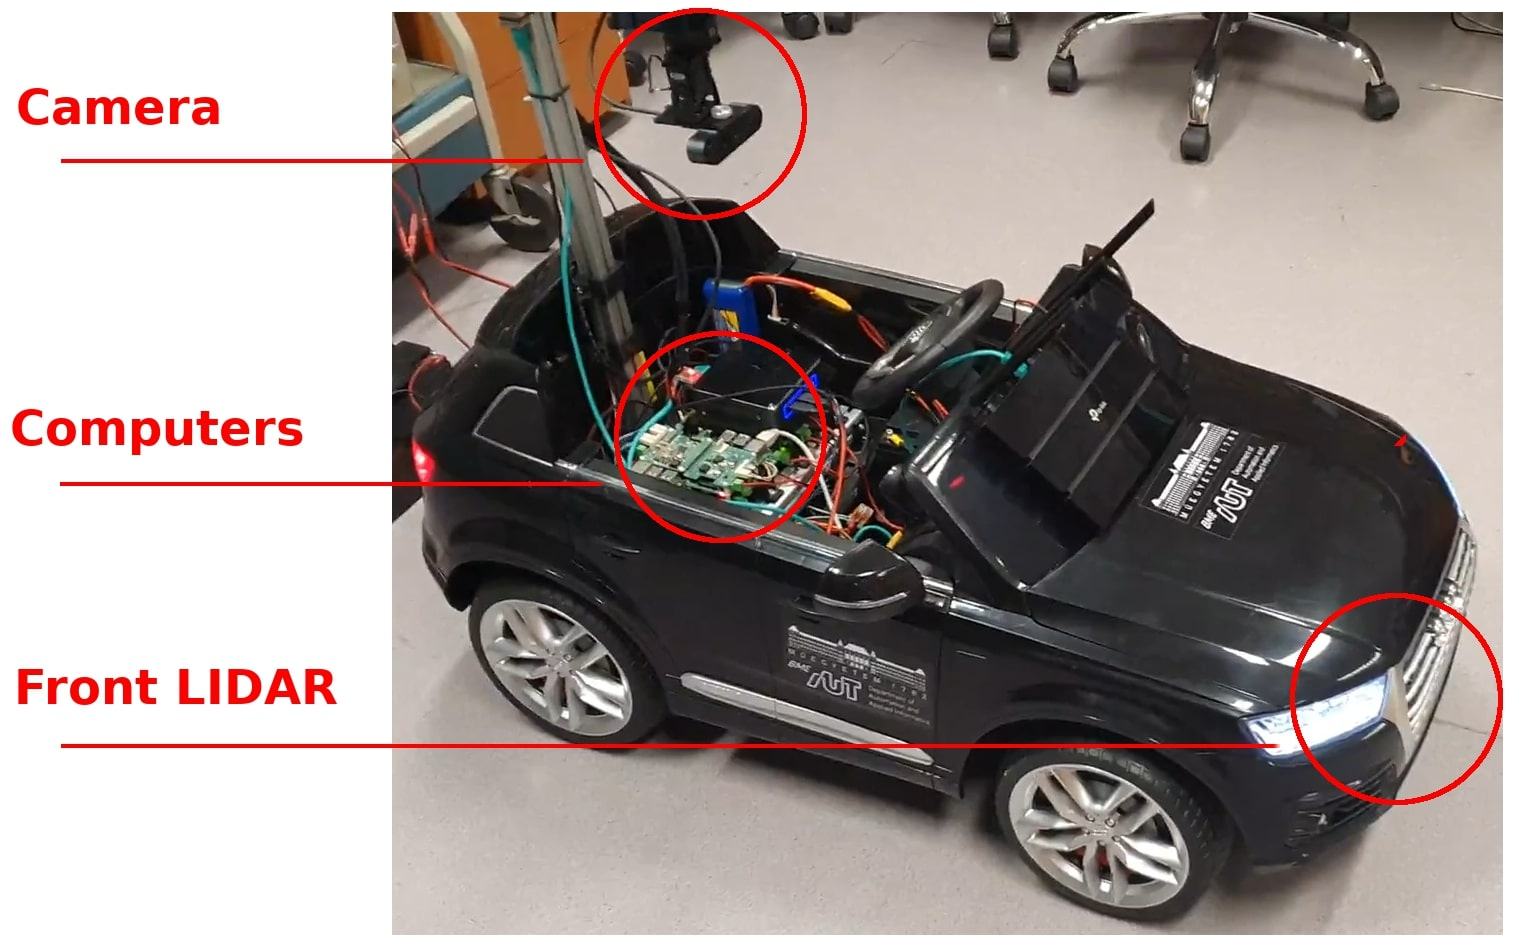
\includegraphics[height=80mm]{figures/raw/car_setup_front.png}
    \caption{The car setup (front side)}
    \label{car_setup_front}
\end{figure}

Amongst others, the car is equipped with a front, a rear and a top LIDAR, a camera, inertial sensors, ultrasonic distance sensors, several Raspberry Pi-s and an Intel NUC computer.

\begin{figure}[!ht]
    \centering
    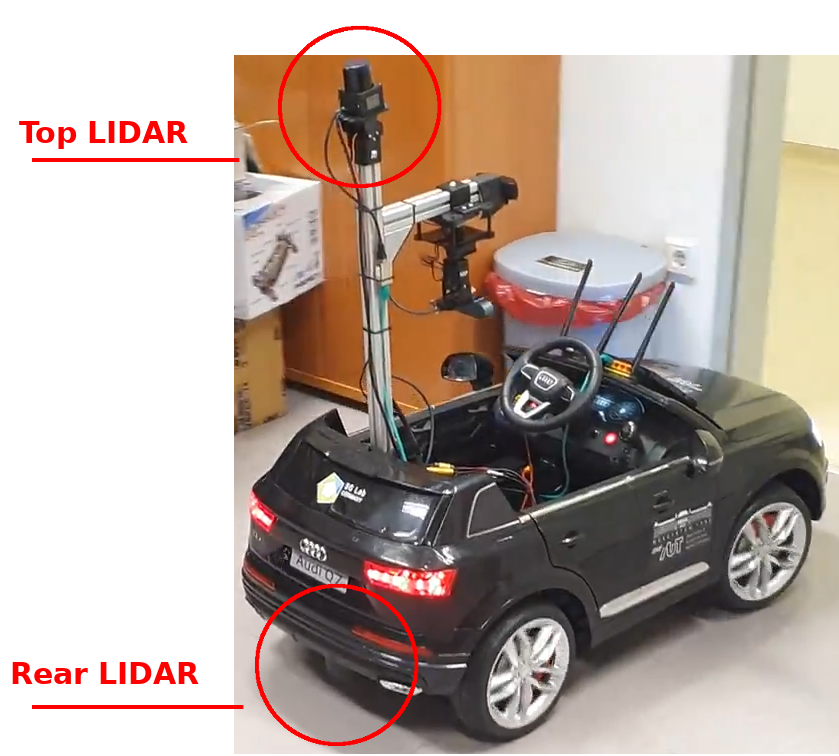
\includegraphics[height=100mm]{figures/raw/car_setup_rear.png}
    \caption{The car setup (rear side)}
    \label{car_setup_rear}
\end{figure}

The vehicle supports the development and testing of multiple smaller projects (mapping and navigation algorithms, control modules, etc.), all contributing to the car becoming more and more able to drive itself. For these sub-projects, the above mentioned sensors are all needed, later I will explain them in detail. These sensors and computers provide a good hardware base for the project, but they are not all that's necessary. A project of this complexity cannot be maintained without a reliable and robust software framework to build upon. This framework is ROS.

\subsection{About ROS}

\begin{quote}
"The Robot Operating System (ROS) is a \textbf{set of software libraries} and tools that help you build robot applications. From drivers to state-of-the-art algorithms, and with powerful developer tools, ROS has what you need for your next robotics project. And it's all \textbf{open source}."
\end{quote}

The above description is quoted\footnote{As the short descriptions on ROS pages are pretty straightforward, I am going to quote from them whenever possible.} from their website \cite{ros}. Short as it may be, their description does point out that ROS is a software framework for robotic applications. Wikipedia also has a brief and comprehensible article \cite{wiki_ros} about ROS, in which it states that:

\begin{quote}
"Although ROS is \textbf{not an operating system}, it provides services designed for a heterogeneous computer cluster such as hardware abstraction, low-level device control, implementation of commonly used functionality, message-passing between processes, and package management. Running sets of ROS-based processes are represented in a \textbf{graph architecture} where processing takes place in nodes that may receive, post and multiplex sensor data, control, state, planning, actuator, and other messages. Despite the importance of reactivity and low latency in robot control, ROS itself is not a real-time OS (RTOS). It is possible, however, to integrate ROS with real-time code."
\end{quote}

So what is ROS exactly? It is a framework that helps building robot applications. It is basically a large set of software components with an own build system. It is not an operating system, therefore it needs one under it. Although it may be installed on Debian and Windows 10 as well, its main target OS is Ubuntu. For this reason, the chosen OS for the computers in the project became Ubuntu (versions Artful and Bionic are supported).

All ROS applications have a graph architecture, meaning that they are considered as a set of separate processes (nodes) that are connected via messages. These message are published on topics, which are message bus names. ROS defines some popular message types, but supports custom messages as well. The communication through messages is based on the publish-subscribe model, a publisher provides some data on a topic in the form of messages that all subscribed nodes can read. The implementation of the message-passing, the used networks layer and the transmission and reception of the messages are hidden from the application. ROS handles the delivery between different processes and even different hosts.

What ROS guarantees is a stable build system and architecture that helps developers create multi-process applications relatively easy, with reliable message-passing over a configurable transport layer (TCP by default). However, these features would not be enough for developers to consider ROS a relevant candidate for a robotic application framework, easy-to-integrate tools and a detailed documentation are also necessary. Fortunately, ROS does include these.

Its documentation is comprehensible and covers most topics that developers may need to look into. Besides that, a large series of tutorials are also available on their website about getting started with ROS and building simple applications, and also about deeper topics that give major insight to the reader about how ROS tools and features can be used effectively. These tutorials usually demonstrate given features using example applications that are also available for installing.

\subsection{Useful ROS tools}
ROS comes with numerous tools that are plug-and-play compatible any applications, due to that fact that ROS apps are just a set of independent nodes --- once opened, these tools become nodes in the ROS graph and they can communicate with the other nodes via messages.

Most of these tools enable the developer to monitor the ROS graph, the existing nodes and the connections among them. Let me mention a few of these programs that proved themselves elementary during working with ROS.

The first one is rqt\_graph \cite{ros_rqt_graph}, which is GUI tool for visualizing the ROS graph --- the nodes and the message connections among them. Figure \ref{rqt_graph} shows part of the \textit{vr-car} ROS graph represented using rqt\_graph. The nodes are shown in the ellipses, and the arrows among them are the topics, on which the messages are sent.

\begin{figure}[!ht]
	\centering
	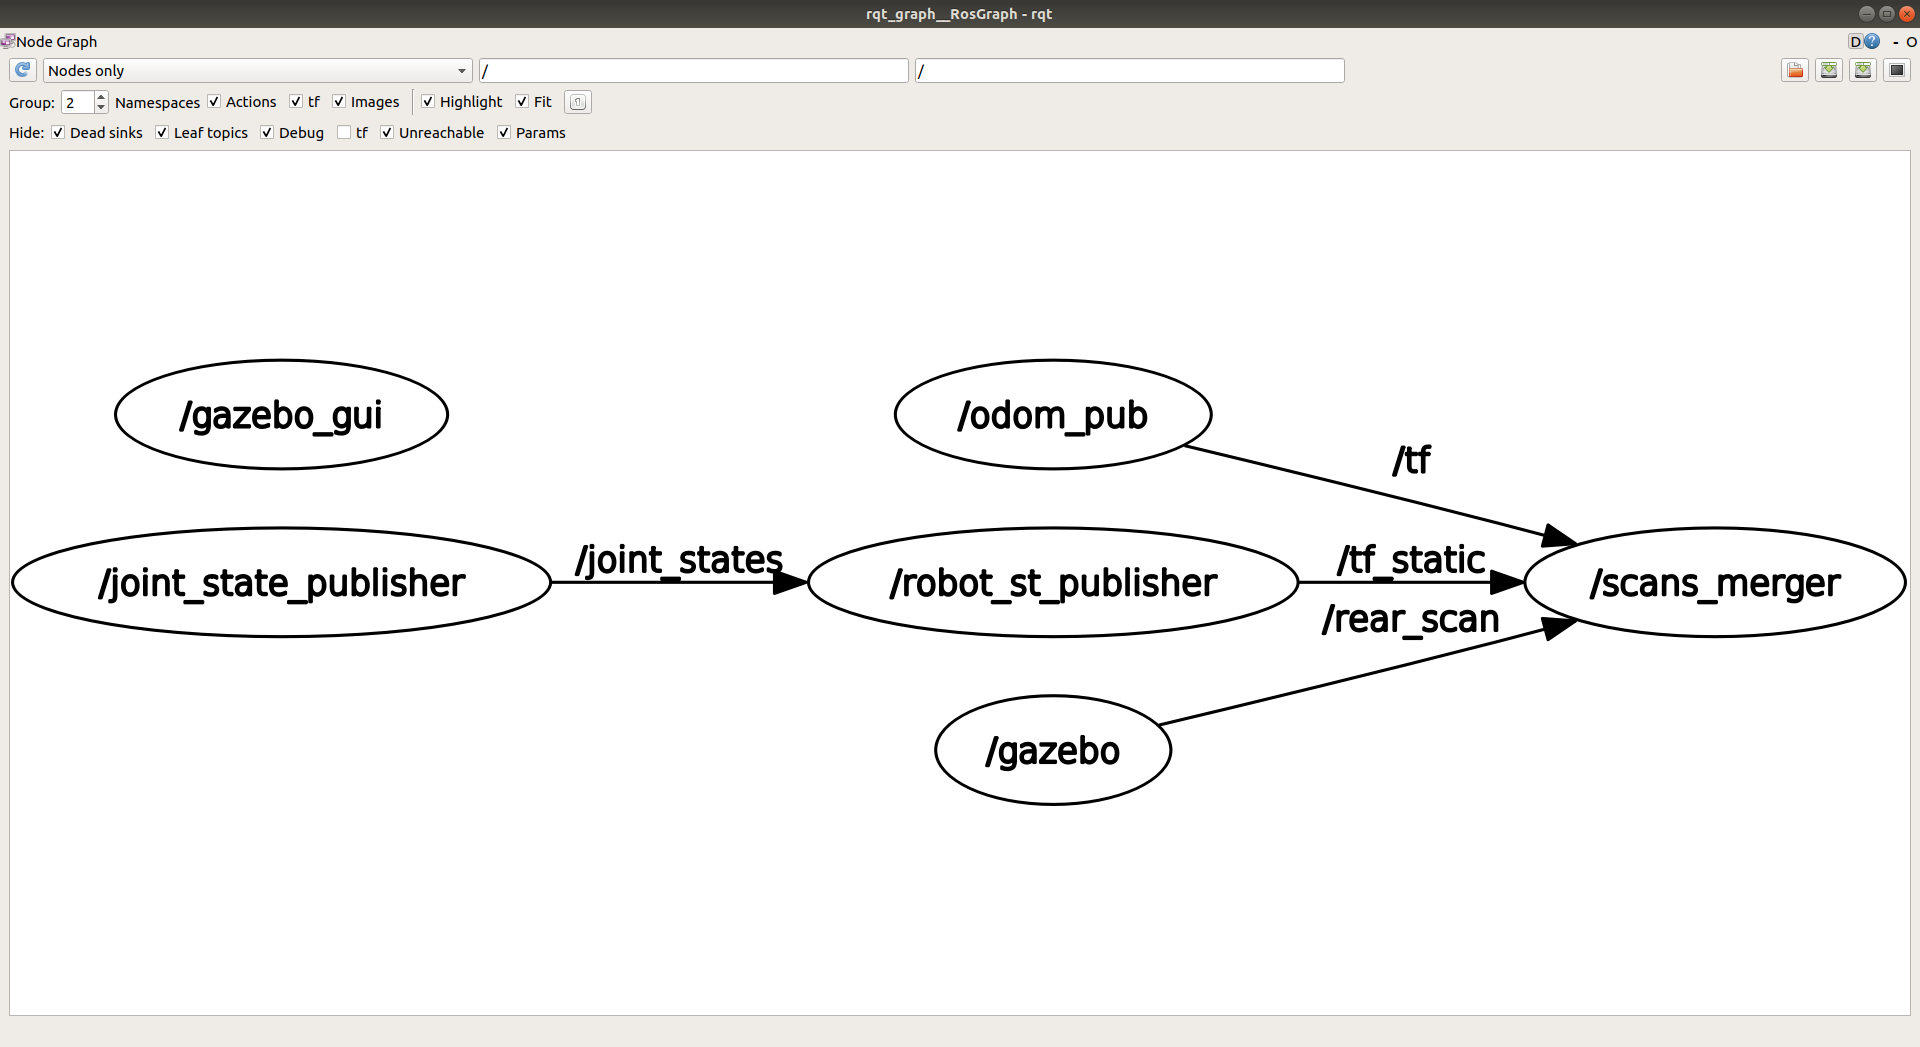
\includegraphics[width=\textwidth]{figures/raw/rqt_graph.png}
	\caption{Visualizing the ROS graph using rqt\_graph}
	\label{rqt_graph}
\end{figure}

A useful command-line tool is rostopic \cite{ros_rostopic}, which may be used to list, search and monitor message topics. For example executing \textit{rostopic list} while the \textit{vr-car} project is running produces the following output:

\begin{minipage}{\textwidth}
\begin{lstlisting}[language=bash]
/Global_planner_wrapper/plan
/camera1/VRcar/camera
/camera1/VRcar/camera/compressed
/camera1/VRcar/camera/compressed/parameter_descriptions
/camera1/VRcar/camera/compressed/parameter_updates
/camera1/VRcar/camera/compressedDepth
/camera1/VRcar/camera/compressedDepth/parameter_descriptions
/camera1/VRcar/camera/compressedDepth/parameter_updates
/camera1/VRcar/camera/theora
/camera1/VRcar/camera/theora/parameter_descriptions
/camera1/VRcar/camera/theora/parameter_updates
/camera1/camera_info
/camera1/parameter_descriptions
/camera1/parameter_updates
/clicked_point
/clock
/front_scan
/gazebo/link_states
/gazebo/model_states
/gazebo/parameter_descriptions
/gazebo/parameter_updates
/gazebo/set_link_state
/gazebo/set_model_state
/initialpose
/joint_states
/lidar_pcl
/lidar_scan
/move_base/global_costmap/costmap
/move_base/global_costmap/costmap_updates
/move_base/local_costmap/costmap
/move_base/local_costmap/costmap_updates
/move_base_simple/goal
/odom
/particlecloud
/path_planner/path_visualization
/path_planner/path_visualization_array
/rear_scan
/rosout
/rosout_agg
/static_grid_updates
/tf
/tf_static
/vrcar/filtered_control
\end{lstlisting}
\end{minipage}

For robotic applications, coordinate transformations and frame tracking in time are essential. Fortunately, ROS has an off-the-shelf solution for coordinate frame handling, this program is called tf. Its documentation \cite{ros_tf} briefly explains that

\begin{quote}
"tf is a package that lets the user keep track of multiple coordinate frames over time. tf maintains the relationship between coordinate frames in a tree structure buffered in time, and lets the user transform points, vectors, etc between any two coordinate frames at any desired point in time."
\end{quote}

And for visualizing the tf tree, rqt \cite{ros_rqt} may be used.

\begin{figure}[!ht]
	\centering
	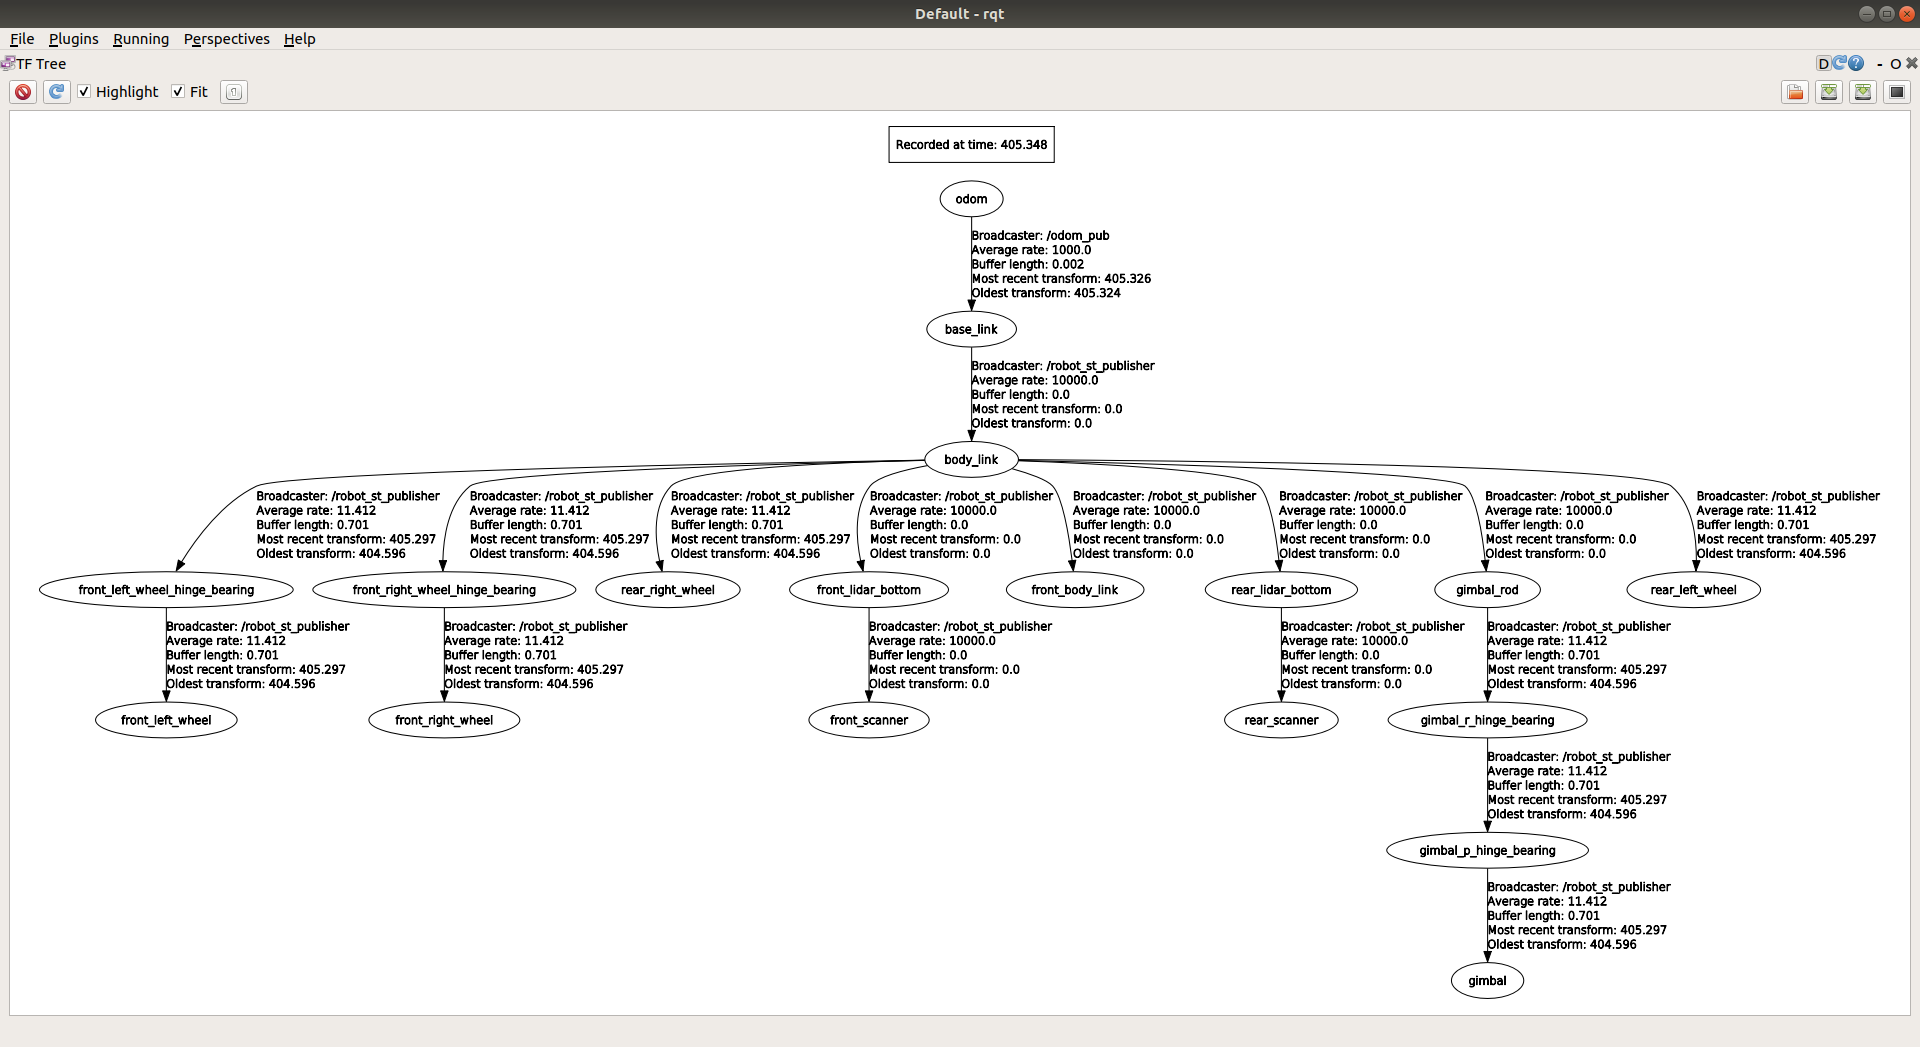
\includegraphics[width=\textwidth]{figures/raw/rqt.png}
	\caption{Visualizing the tf tree using rqt}
	\label{rqt_graph}
\end{figure}

In many cases, algorithm testing consists of various iterations, and it is handy to provide the program the same inputs over and over. For this purpose, ROS has a tool called rosbag \cite{ros_rosbag}, which is able to record and play back messages. This way, the whole ROS graph may be simulated by replaying the node outputs. Debugging algorithms is much easier using rosbag recordings, than having to recreate the same situations running the actual nodes.

The tools mentioned above were programs that help developers to monitor or interfere with the ROS graph and node communications. However, there are standalone applications, too, that are, in a way, independent from the ROS graph overall, they work like regular graph nodes that have certain inputs and outputs.

One of most essential standalone program is rviz \cite{ros_rviz}, a 3D visualization tool. rviz supports a wide range of elements that it can display (camera images, maps, markers, point clouds, robot models, etc.), and the developers also have the option to implement custom display plugins for their own types.

\begin{figure}[!ht]
	\centering
	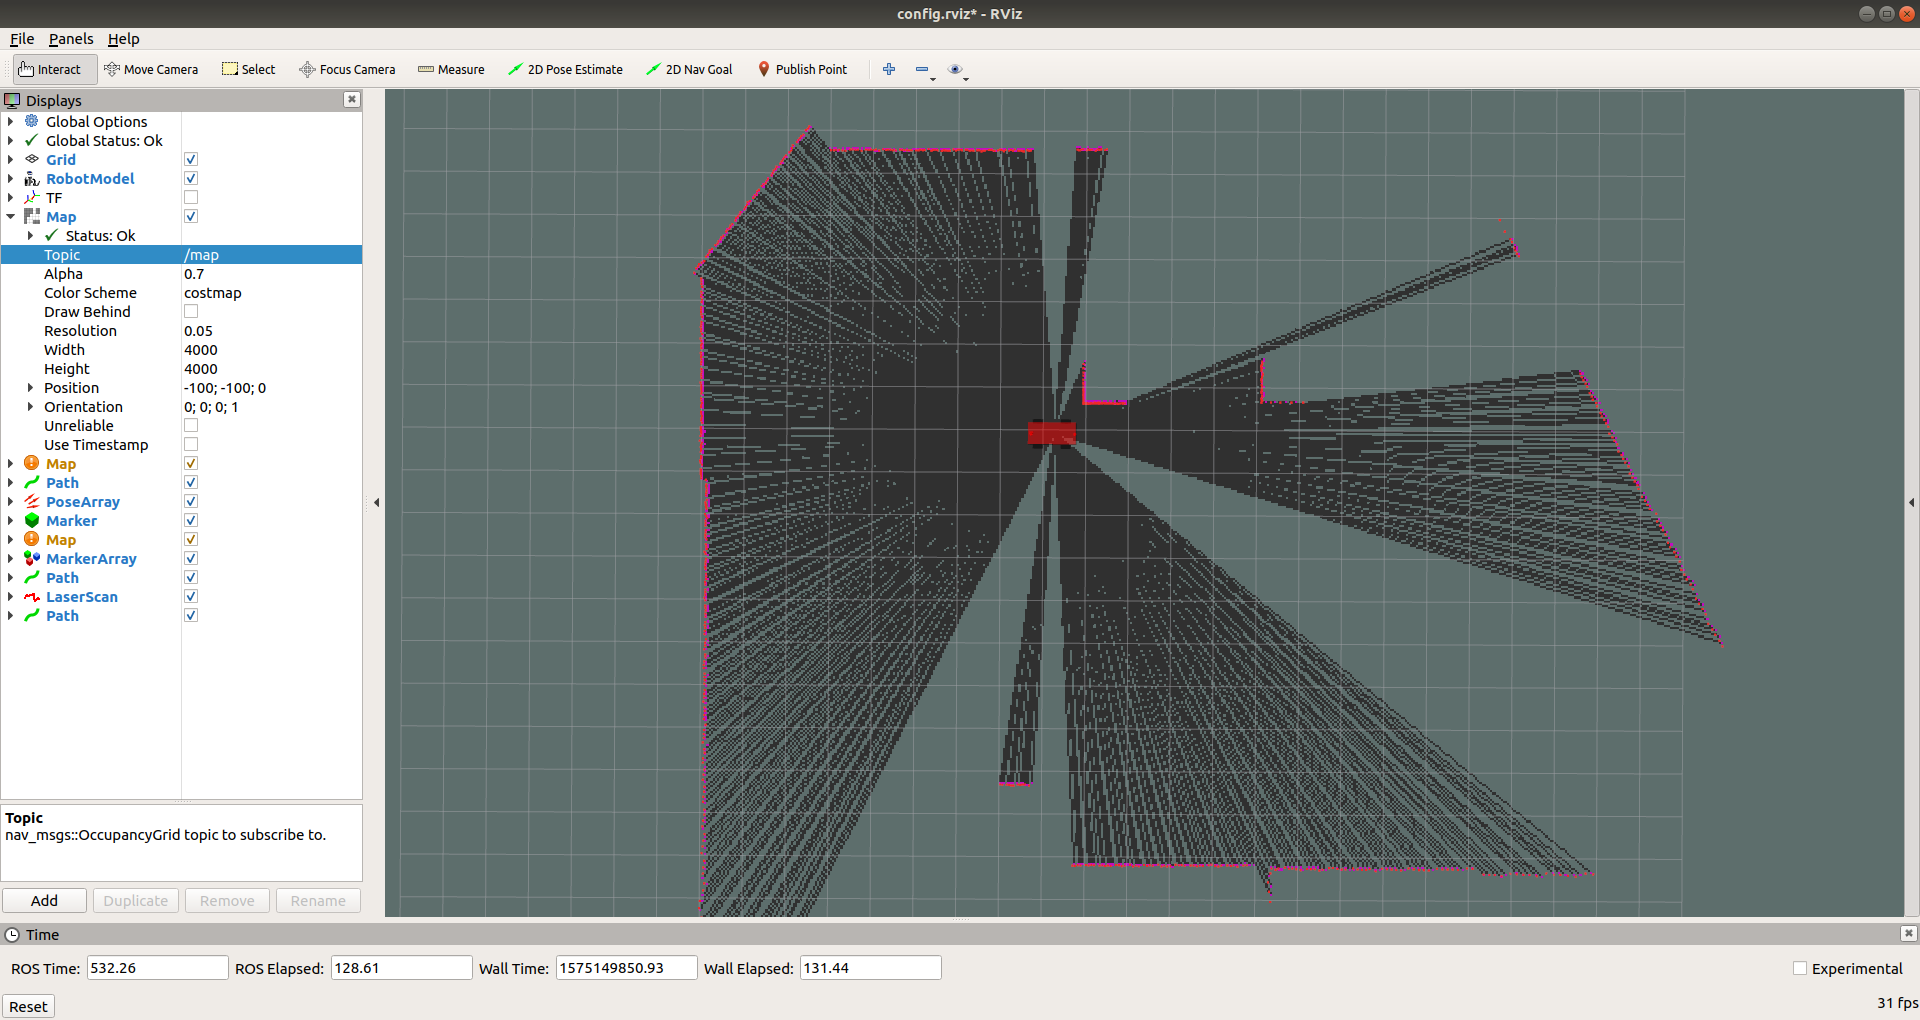
\includegraphics[width=\textwidth]{figures/raw/rviz.png}
	\caption{rviz}
	\label{rviz}
\end{figure}

For vehicle applications such as the \textit{vr-car} project, the typical displayed types are robot models, odometry, trajectories and maps. Just imagining the simplest car driving project we can, displaying the car's position and orientation could be quite useful. Unsurprisingly, rviz supports the visualization of vehicle odometry \cite{ros_rviz_Odometry}, and according to its documentation:

\begin{quote}
"The Odometry display accumulates a nav\_msgs/Odometry \cite{ros_msg_Odometry} message over time, showing them as arrows."
\end{quote}

So one of the nodes in the project's graph needs to publish the odometry messages, and no further coding is needed, rviz may be opened and odometry will be displayed.

Testing in real life, with the real target host may be difficult and expensive. My diploma project is a perfect example for this, because the test car that operates as the host for the ROS nodes was very rarely accessible for me, as I was developing the project from home. Therefore, having to test my algorithm with the actual \textit{vr-car} vehicle would have been a struggle. Fortunately, Gazebo \cite{gazebo}, which is an open-source 3D robotics simulator, can be connected to ROS easily. With the help of this software, I was able to simulate the car (alongside the sensors and actuator fixed on it) on my computer. What Gazebo provides according to their website is

\begin{quote}
"a robust physics engine, high-quality graphics, and convenient programmatic and graphical interfaces."
\end{quote}

Simulating in Gazebo is relatively more difficult than visualizing in rviz. At every simulation start, Gazebo needs to be given a world describing the simulation environment, and objects to place in the world (e.g. in the simulation represented in Figure \ref{gazebo} the world consists of the boxes, while the object placed in the world is the red car).

\begin{figure}[!ht]
	\centering
	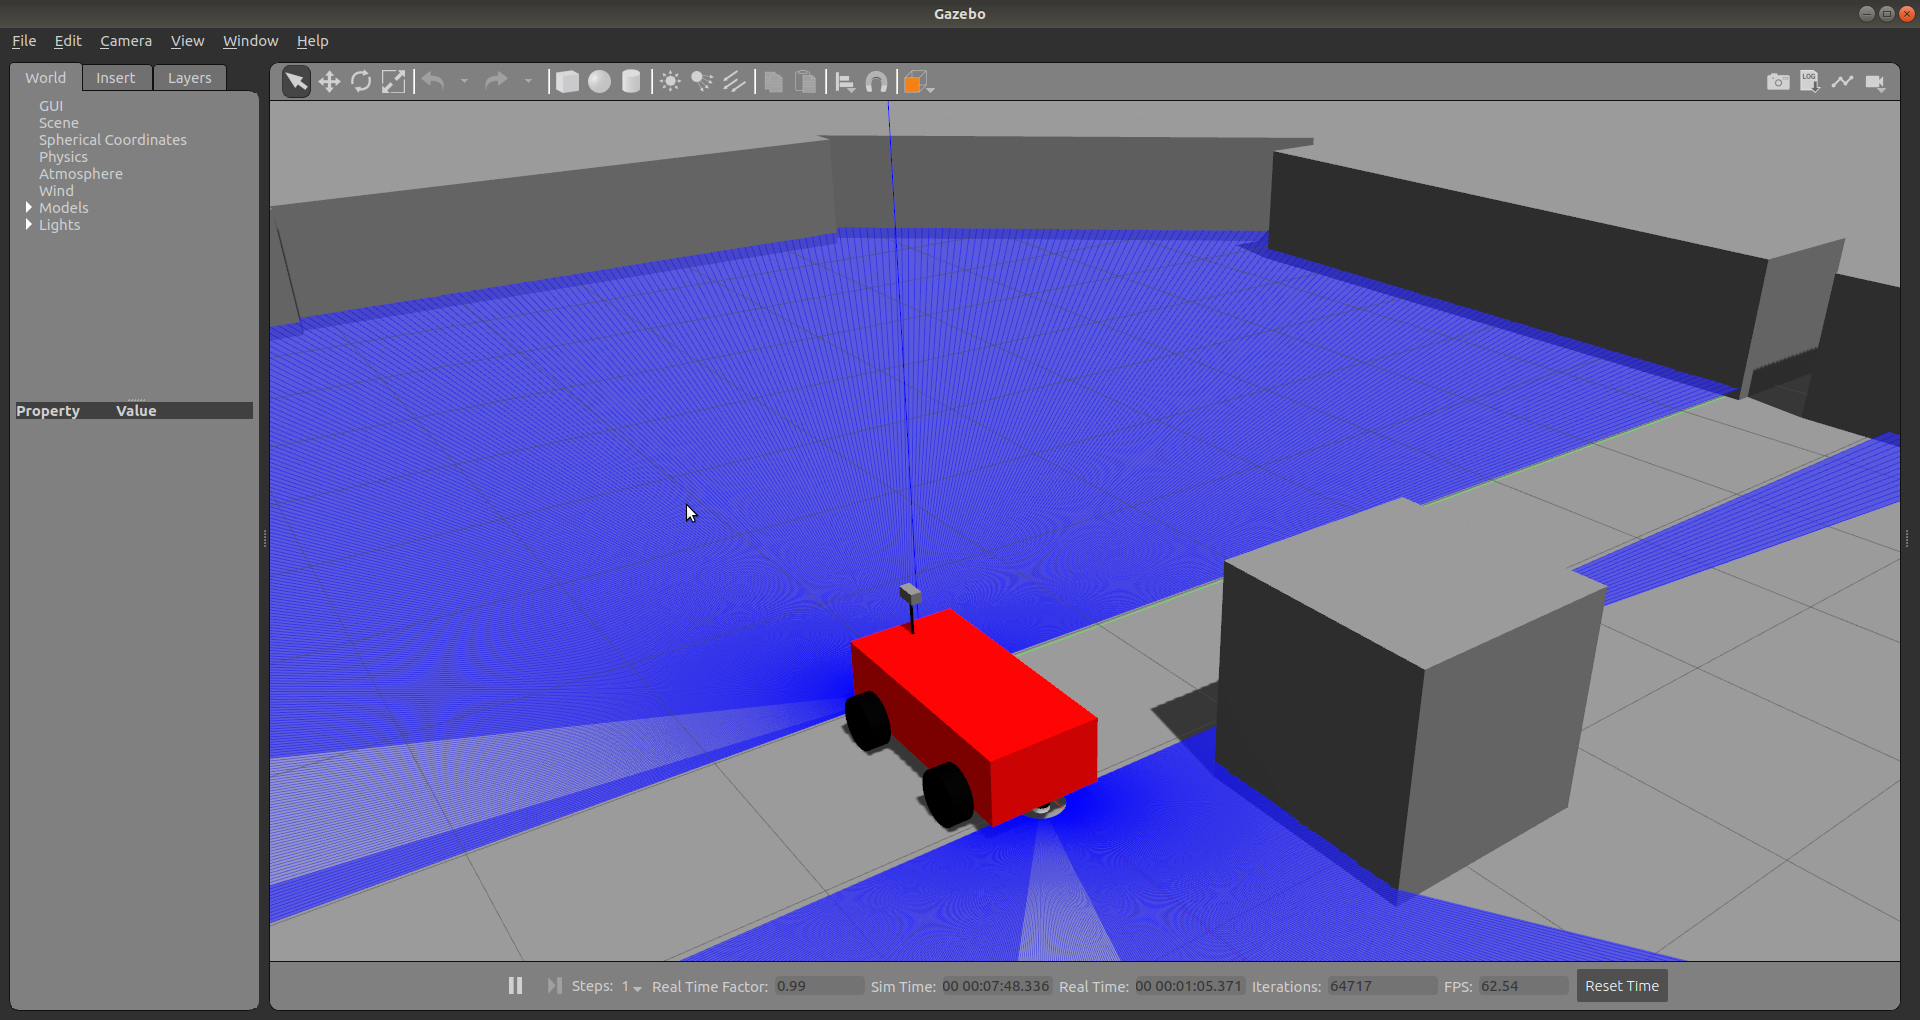
\includegraphics[width=\textwidth]{figures/raw/gazebo.png}
	\caption{Gazebo}
	\label{gazebo}
\end{figure}

The simulated world is defined by an SDF file. Quoting from their website \cite{sdf}:

\begin{quote}
"SDF is an XML format that describes objects and environments for robot simulators, visualization, and control. Originally developed as part of the Gazebo robot simulator, SDF was designed with scientific robot applications in mind. Over the years, SDF has become a stable, robust, and extensible format capable of describing all aspects of robots, static and dynamic objects, lighting, terrain, and even physics."
\end{quote}

In the \textit{vr-car} project, the car in the simulation is defined by Unified Robot Description Format (URDF) files \cite{ros_urdf}. These are also XML descriptors that define the structure of an object by links and joints. A basic URDF file containing a single cylinder looks like the following (the example is taken from one of the URDF tutorials \cite{ros_urdf_tutorials} provided by ROS):

\begin{minipage}{\textwidth}
\begin{lstlisting}[language=XML]
<?xml version="1.0"?>
<robot name="mokifej_foni">
  <link name="base_link">
    <visual>
      <geometry>
        <cylinder length="0.6" radius="0.2"/>
      </geometry>
    </visual>
  </link>
</robot>
\end{lstlisting}
\end{minipage}

Both the SDF world and the URDF models can be opened, edited and saved in Gazebo, thus making the creation and update of these files easy. These models were already created by another member of the \textit{vr-car} project, so I was able to simulate the car without any difficulty or extra work, which was a great help during the development of my algorithms.

In the next sections I am going to explain the ROS graph and the message-passing between nodes using a simplified model of the \textit{vr-car} project, while also describing the features of the application.

\subsection{Remote drive}
The first (and probably simplest to comprehend) feature of the car is the ability to control it remotely, using either a PC keyboard, a joystick or a set of racing wheel and pedals.

In order to make this possible, the car definitely needed a node that controls the car's actuators according to an input actuation. For simplicity, let's assume that this input actuation (a ROS message) contains a target speed and wheel angle that the module has to handle as a reference. Having direct control of the car's motors (the accelerator DC motor and the steering servo) and of the necessary sensors (e.g. a rotary encoder for measuring speed) the control is manageable.

Besides this control module, the graph contains another node, that reads driver interactions (key strokes, joystick state or steering wheel and pedal positions), converts these to driver commands (target actuations) and publishes the correspondent messages that the control node listens to. Note, that these input nodes are implemented separately for the input types --- there is a module for keyboard input, one for handling the joystick and a third one for reading the racing wheel and pedal data\footnote{The racing wheel and the throttle and brake pedals are actually handled on a separate Windows host, and their positions are forwarded to another host running ROS.}.

With one input module being active, the graph now contains two processes --- the input and the control nodes. These two nodes are communicating through a message that contains speed and wheel angle reference values.

\subsection{\textit{vr-drive}}
Another feature of the car is that the user drive it using one of the input methods listed above while 'seeing what the car sees'. This is implemented by reading the video stream from the camera fixed on the vehicle and transferring it to the user's PC. The user can see the images via an Oculus Rift VR headset. To make it more realistic, the camera on the car is moved in a way that it follows the user's head movements.

\subsection{2D mapping}
As figures \ref{car_setup_front} and \ref{car_setup_rear} show, the car is equipped with a front and a rear 2-dimensional, 360 degree LIDAR. The sensors are hard to see because they are fixed under the chassis. The reason for them being hidden is that they are meant to detect low-height objects as well, therefore they could not have been placed on the top of the car, which would be the usual placement of LIDARs. But as the front LIDAR cannot see backward effectively because it is covered by the wheels (and the same goes for the rear LIDAR looking forward), both LIDARs are needed in order to have a 360 degree view angle. But because the two LIDARs are placed on two different locations on the car, creating one map from their measured values is not trivial. To solve this issue, a special node called \textit{scans\_merger} has been added to project, with the task to merge the scan data from the front and rear LIDARs, thus creating a joined scan.

This scan needs to be evaluated and and kept track over time, while the car is moving, in order to create a map from them. This algorithm could have been initialized as part of the project, but a popular ROS package, gmapping \cite{ros_gmapping} is able to do that outstandingly\footnote{The advantages and drawbacks of gmapping will be discussed in Section \ref{chap:mapping}.}.

\subsection{3D mapping}

\begin{figure}[!ht]
	\centering
	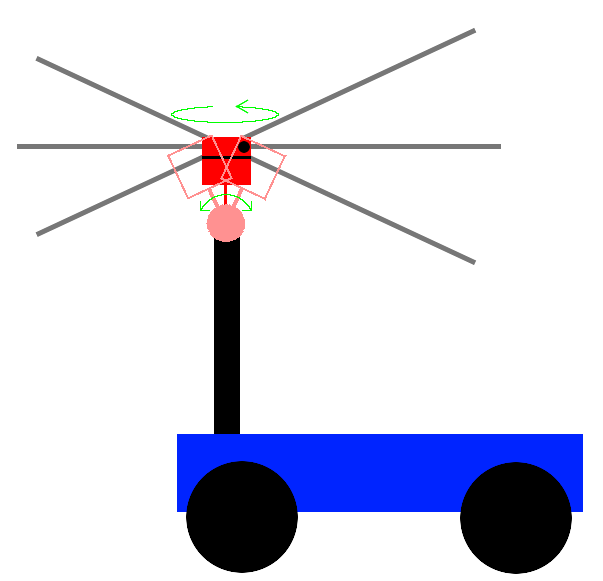
\includegraphics[height=72mm]{figures/raw/3D_lidar.png}
	\caption{Creating a 3D map by tilting a 2D LIDAR}
	\label{tilt_lidar}
\end{figure}

3D mapping is implemented using the top LIDAR, which is also a 2-dimensional, 360 degree sensor, but it is placed on a gimbal, and is tilted forward and backward with ~0.5 Hz frequency. Because of the tilting movement, the LIDAR scans a different plane in every step. And merging these planes creates a 3D map (see Figure \ref{tilt_lidar}).

\subsection{Navigation}
The project has a goal to make the car able to navigate from its actual position to a desired target position in the map. In order to do that, it needs a reliable map of its environment. As I mentioned earlier, gmapping produces a good-quality map, therefore the navigation algorithm uses that as its base. Looking at the navigation node as a black box (other members of the project have implemented and are still working on it, its internal logic is not relevant for my diploma project), it receives a destination pose in a ROS message, and produces a path in another. Both the input and output messages are standard ROS messages that I will explain in detail later. For providing the destination pose for the algorithm, there exists several possibilities, but one of the most straightforward method is through rviz. The visualization tool is not only capable of displaying content, but it has a feature that the user can select a '2D Nav Goal' in the view, and the selected pose will be sent out on a specific topic into the graph. A very effective and elegant way is to combine the map drawing with this feature for creating an interface that enables the user to decide where the next destination pose should be, by clicking somewhere in the map. Needless to say, giving a target position for the navigation node is implemented using this method.

\tikzset{
	base_node/.style    = {rectangle, rounded corners, draw=black,
		minimum width=4.5cm, minimum height=1cm,
		text centered, font=\sffamily},
	inout_node/.style   = {base_node, fill=blue!30},
	vr_car_node/.style  = {base_node, fill=orange!15},
	decoration={brace},
	tuborg/.style={decorate},
	tubnode_left/.style={midway, left=2pt},
	tubnode_right/.style={midway, right=2pt}
}

\begin{figure}[!ht]
	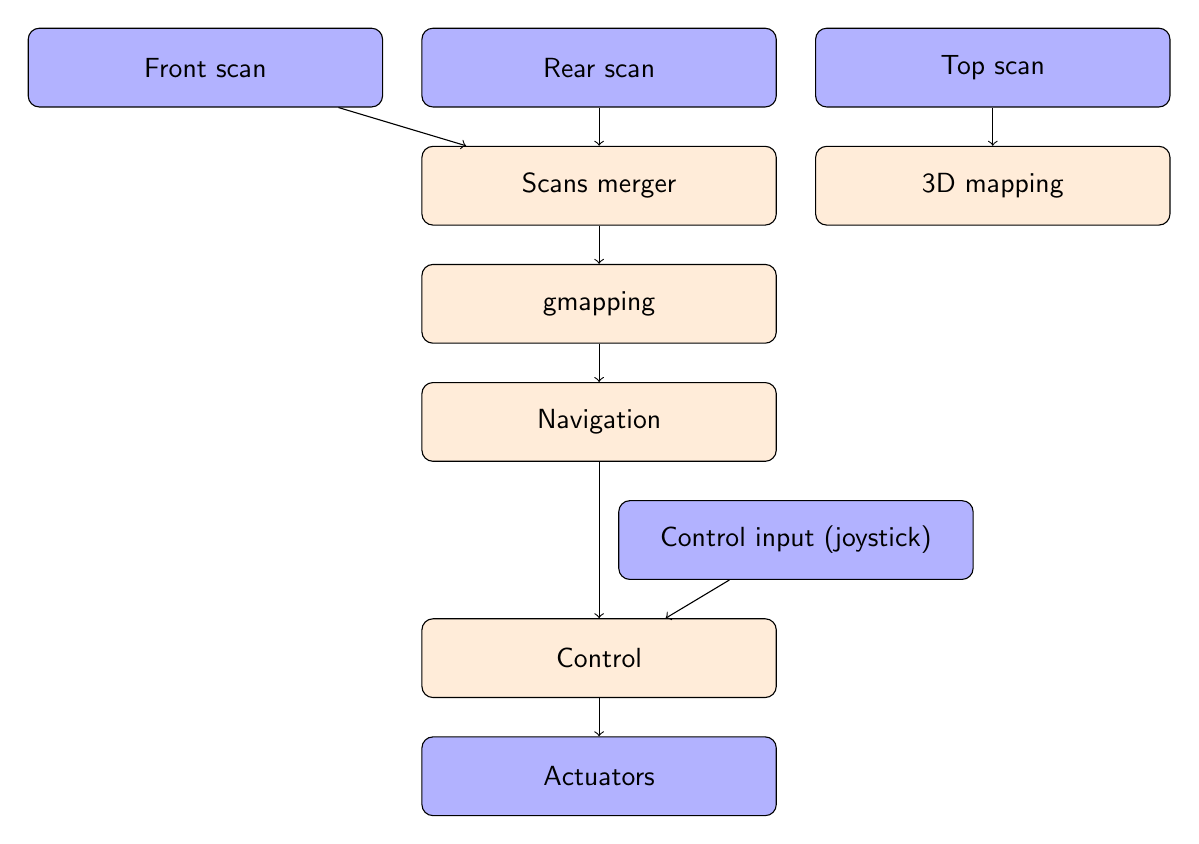
\begin{tikzpicture}[
	node distance=1.5cm,
	every node/.style={fill=white, font=\sffamily}, align=center]
	% Input nodes
	\node (front_scan)       [inout_node]                                      {Front scan};
	\node (rear_scan)        [inout_node, xshift=5.0cm]                        {Rear scan};
	\node (top_scan)         [inout_node, xshift=10.0cm]                       {Top scan};
	\node (control_input)    [inout_node, xshift=7.5cm, yshift=-6.0cm]         {Control input (joystick)};
	% Active nodes
	\node (scans_merger)     [vr_car_node, below of=rear_scan]                 {Scans merger};
	\node (gmapping)         [vr_car_node, below of=scans_merger]              {gmapping};
	\node (navigation)       [vr_car_node, below of=gmapping]                  {Navigation};
	\node (3d_mapping)       [vr_car_node, below of=top_scan]                  {3D mapping};
	\node (control)          [vr_car_node, below of=navigation, yshift=-1.5cm] {Control};
	% Output node
	\node (actuators)        [inout_node, below of=control]                    {Actuators};
	% Connections
	\draw[->]     (front_scan) -- (scans_merger);
	\draw[->]      (rear_scan) -- (scans_merger);
	\draw[->]   (scans_merger) -- (gmapping);
	\draw[->]       (gmapping) -- (navigation);
	\draw[->]  (control_input) -- (control);
	\draw[->]     (navigation) -- (control);
	\draw[->]        (control) -- (actuators);
	\draw[->]       (top_scan) -- (3d_mapping);
	\end{tikzpicture}
	\caption{The original \textit{vr-car} graph}
	\label{original_vr_car_graph}
\end{figure}

Now that the main features of the \textit{vr-car} has been listed and briefly explained, let me introduce what my part of the project was, and how it fits into the existing graph. So far, the graph consists of the nodes represented in Figure \ref{original_vr_car_graph}. Note, that this image is a simplified version of the actual \textit{vr-car} graph, it does not contain all the existing nodes, and some nodes have been merged into one for the sake of simplicity.

\subsection{Avoiding moving obstacles}
My task as a diploma project was to design, implement and tune two nodes, that embed themselves into the existing graph.

The first one is a mapping node. While there are numerous mapping implementations available in ROS (see gmapping for one example), none of them handles moving objects correctly (I am providing a detailed reasoning in Section \ref{chap:mapping}). So the goal of the mapping node was to separate the static points from the moving objects in the map.

The other node was a local trajectory planner node, that (based on the mapping nodes output of static and dynamic objects) performs local obstacle avoidance considering not only the position but also the velocities of the surrounding obstacles.

\tikzset{
	base_node/.style    = {rectangle, rounded corners, draw=black,
		minimum width=4.5cm, minimum height=1cm,
		text centered, font=\sffamily},
	inout_node/.style   = {base_node, fill=blue!30},
	common_node/.style  = {base_node, fill=orange!15},
	dynamic_node/.style = {base_node, fill=green!30},
	static_node/.style  = {base_node, fill=red!30},
	decoration={brace},
	tuborg/.style={decorate},
	tubnode_left/.style={midway, left=2pt},
	tubnode_right/.style={midway, right=2pt}
}

\tikzset{
	base_node/.style    = {rectangle, rounded corners, draw=black,
		minimum width=4.5cm, minimum height=1cm,
		text centered, font=\sffamily},
	inout_node/.style   = {base_node, fill=blue!30},
	vr_car_node/.style  = {base_node, fill=orange!15},
	added_node/.style   = {base_node, fill=green!30},
	decoration={brace},
	tuborg/.style={decorate},
	tubnode_left/.style={midway, left=2pt},
	tubnode_right/.style={midway, right=2pt}
}

\begin{figure}[!ht]
	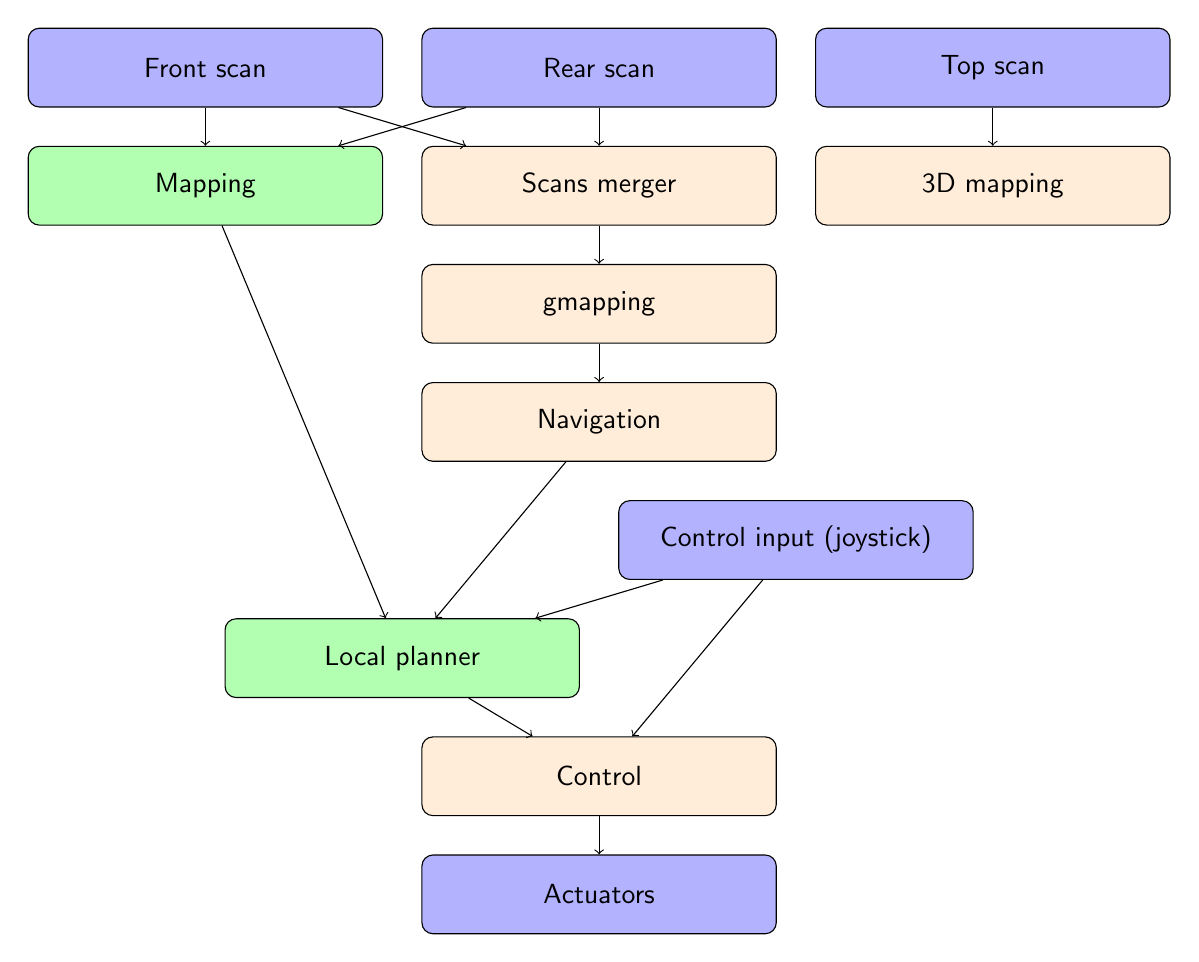
\begin{tikzpicture}[
	node distance=1.5cm,
	every node/.style={fill=white, font=\sffamily}, align=center]
	% Input nodes
	\node (front_scan)       [inout_node]                                                {Front scan};
	\node (rear_scan)        [inout_node, xshift=5.0cm]                                  {Rear scan};
	\node (top_scan)         [inout_node, xshift=10.0cm]                                 {Top scan};
	\node (control_input)    [inout_node, xshift=7.5cm, yshift=-6.0cm]                   {Control input (joystick)};
	% Active nodes
	\node (scans_merger)     [vr_car_node, below of=rear_scan]                           {Scans merger};
	\node (gmapping)         [vr_car_node, below of=scans_merger]                        {gmapping};
	\node (navigation)       [vr_car_node, below of=gmapping]                            {Navigation};
	\node (3d_mapping)       [vr_car_node, below of=top_scan]                            {3D mapping};
	\node (control)          [vr_car_node, below of=navigation, yshift=-3.0cm] 			 {Control};
	% Added nodes
	\node (mapping)          [added_node, below of=front_scan]                           {Mapping};
	\node (local_planner)    [added_node, below of=mapping, xshift=2.5cm, yshift=-4.5cm] {Local planner};
	% Output node
	\node (actuators)        [inout_node, below of=control]                              {Actuators};
	% Connections
	\draw[->]     (front_scan) -- (scans_merger);
	\draw[->]      (rear_scan) -- (scans_merger);
	\draw[->]   (scans_merger) -- (gmapping);
	\draw[->]       (gmapping) -- (navigation);
	\draw[->]  (control_input) -- (control);
	\draw[->]        (control) -- (actuators);
	\draw[->]       (top_scan) -- (3d_mapping);
	% Added connections
	\draw[->]     (front_scan) -- (mapping);
	\draw[->]      (rear_scan) -- (mapping);
	\draw[->]        (mapping) -- (local_planner);
	\draw[->]  (control_input) -- (local_planner);
	\draw[->]     (navigation) -- (local_planner);
	\draw[->]  (local_planner) -- (control);
	\end{tikzpicture}
	\caption{The modified \textit{vr-car} graph}
	\label{modified_vr_car_graph}
\end{figure}

The \textit{vr-car} graph with the two additional nodes is represented in Figure \ref{modified_vr_car_graph}. The mapping nodes uses the raw front and rear LIDAR scans as its inputs for the map creation. The local trajectory planner node cuts the connection between the Navigation and the Control nodes, because it overrides the pre-calculated path based on the static and dynamic obstacles in the car's environment.